%%
%% cap2.tex
%%
%% Made by Carlos Calcaneo Roldan
%% Login   <calcaneo@jogrant>
%%
%% Started on  Mon Jul 22 15:02:51 2019 Carlos Calcaneo Roldan
%% Last update Time-stamp: <2021-ene-06.miércoles 12:29:37 (Oscar)>
%%

\chapter{Simulaciones Cosmológicas}
\label{chap:2 Sim}
\setcounter{equation}{0}
%%%%%%%%EL Texto Comienza abajo de aquí!

\noindent Las simulaciones cosmológicas son una herramienta esencial para el estudio del Universo. Es el único experimento con el que contamos para reproducir su evolución. Las simulaciones numéricas nos permiten un estudio detallado de formación de estructura no lineal y nos permite hacer conexiones con un Universo simple con alto corrimiento al rojo, con uno complejo como el que se observa en la actualidad.

El trabajo que se realiza va desde el estudio del agrupamiento gravitacional no lineal de materia oscura, formación de grupos de galaxias, interacción de galaxias aisladas y la evolución de gas intergaláctico. Su desarrollo ha permitido un inmenso avance en estas áreas, el cual no era posible antes dado a las limitaciones que existían en el computó \cite{2001NewA....6...79S}.


Con la rápida evolución en el rendimiento de las computadoras y algoritmos numéricos, han nacido múltiples códigos que simulan la formación de estructura del Universo. Muchos de estos códigos se han hecho públicos y libres, lo que ha permitido que el estudio sea mas sencillo para nuevos investigadores o grupos de investigación \cite{2021MNRAS.506.2871S}. El futuro de las simulaciones numéricas esta en hacer mejoras en la precisión y en la fidelidad en la física de las técnicas de modelado.

\newpage

\section{Grandes Simulaciones}

Gracias al desarrollo de códigos y el avance en el hardware de las maquinas modernas, has surgido grandes colaboraciones con la intención de realizar simulaciones cada vez mas grandes. Algunas de ellas son:

%==================================================================================================
%==================================================================================================
%==================================================================================================
\subsubsection{Millennium Simulation}

La Millennium Simulation fue una de las mas grandes simulaciones de N-Cuerpos realizada en el 2005. Esta contenía mas de 10 billones de partículas en una caja de 2 billones de años luz por lado. La simulación se realizó por la Virgo Consortium usando 512 procesadores localizados en el Instituto Max Planck para Astrofísica en Garching, Alemania. Tomo 28 días (~600 horas), consumiendo alrededor de 343,000 horas de tiempo de cpu \cite{2005Natur.435..629S}.

Esta fue la primera simulación parte de una serie de simulaciones relacionadas a volúmenes cosmológicos. En 2008 se realizó una segunda simulación con las misma cosmología, misma estructura de salida y misma cantidad de partículas, pero con una caja 5 veces mas pequeña, lo que aumento la densidad de partículas y por tanto permitió tener una resolución de masa 125 veces mejor.

\begin{figure}[H]
    \centering
    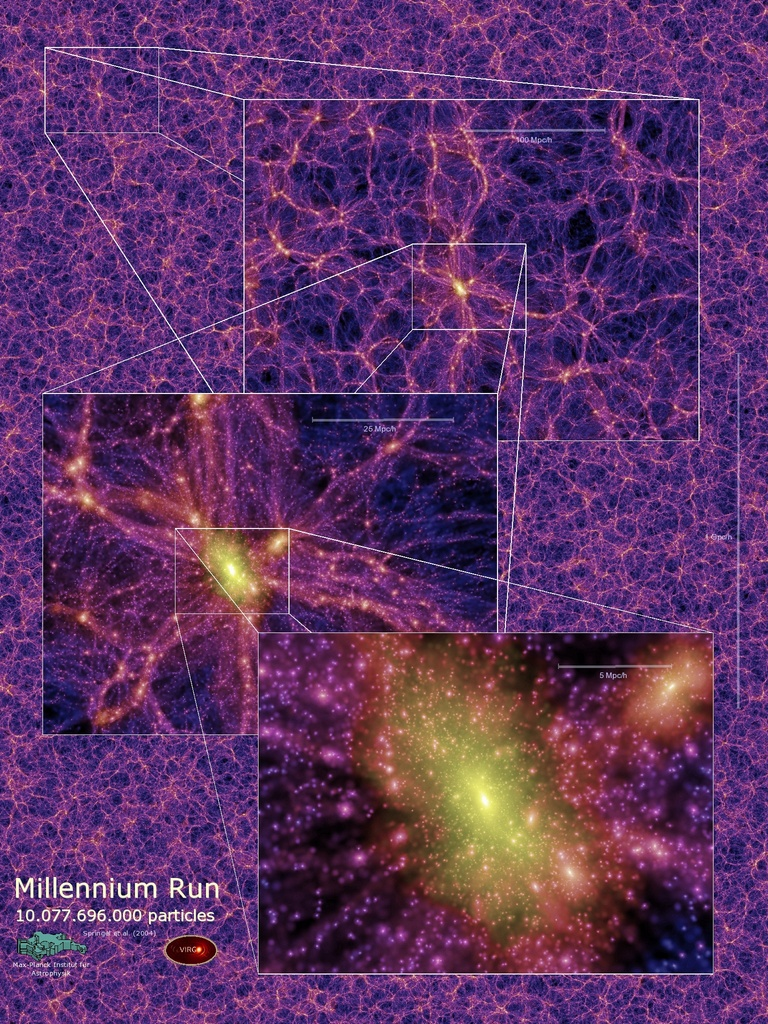
\includegraphics[width = 0.35\linewidth]{Millenium-Sim.jpg}
    \caption[Millennium Simulation Cosmic Web]{Se muestra el mapa de densidad de un corte de $15 Mpc/h$ en redshift $z=0$ de la \textit{Millennium Simulation}. Imagen obtenida de MPA}
    \label{fig:Millennium_Sim}
\end{figure}


%==================================================================================================
%==================================================================================================
%==================================================================================================
\subsubsection{Eagle Simulation}
El proyecto EAGLE (Evolution and Assembly of GaLaxies and their Environments)  es una colaboración de The Virgo Consortium, la cual es una simulación hidrodinámica de gran escala de un Universo de $\Lambda$CDM, el cual tenia como objetivo entender como las galaxias se forman y evolucionan. La mas grande de las simulaciones se realizo con  6.8 billones de partículas, en un volumen de 100 Mpc por lado, conteniendo al menos 10,000 galaxias del tamaño de la vía láctea, la cual tardo mas de un mes y medio de tiempo de computo y una de la mas grandes super-computadoras con 4000 núcleos de procesamiento usando una versión modificada del código de simulación GADGET-2 \cite{2015MNRAS.450.1937C, 2015MNRAS.446..521S}.

La simulación empieza en un Universo todavía muy uniforme (sin formación de estrellas o galaxias) usando parámetros motivados por las observaciones del satélite Plank y del CMB \cite{ 2013ApJS..208...20B, 2020A&A...641A...1P}. Algunos de los parámetros cruciales de la simulación son la densidad de materia oscura, la cual es responsable de la formación de estructura de materia bariónica, así como la constante cosmológica, responsable de la expansión acelerada del Universo.
       
\begin{figure}[H]
    \centering
    \includegraphics[width = 0.45\linewidth]{Eagle-Sim.png}
    \caption[Eagle Simulation Cosmic Web]{Se muestra el mapa de densidad de la Eagle Simulation. Obtenida de \textit{The Eagle Project} }
    \label{fig:Eagle_Sim}
\end{figure}

%==================================================================================================
%==================================================================================================
%==================================================================================================

\section{Interacciones/Gravedad/??? TEMP TITLE}

Para estudiar el comportamiento de de un sistema de partículas, tenemos que simplificarlo la mas posible. Empezando con identificar la fuerza responsable del movimiento de las partículas, en este caso es la gravedad y en específico nos quedamos con la gravedad descrita por Newton \eqref{eq:Gravedad-Newton}. Por tanto, solo requerimos conocer las masas y las posiciones de las partículas.

\begin{equation}
    F = G \frac{m_1 m_2}{r^2}
    \label{eq:Gravedad-Newton}
\end{equation}

Pero como estamos tratando con sistema de $N$ partículas tenemos que considerar la contribución de fuerzas debida al resto de las partículas. Por el teorema de superposición podemos decir que
\begin{equation}
    F_{1} = F_{1,2} +F_{1,3} + \dots + F_{1,N} = \sum_{i=2}^{N} F_{1,i} 
    \label{eq:superposicion}
\end{equation}

Pero también podemos resolver el problema si trabajamos con el potencial
\begin{equation}
    m\nabla \phi(\mathbf{r}) = \mathbf{F}
    \label{eq:potencial-gravitacional}
\end{equation}



 
%==================================================================================================
%==================================================================================================
%==================================================================================================
\section{Simulaciones Cosmológicas}

Si consideramos las dimensiones de nuestra galaxia, podemos calcular el camino medio libre de una estrella antes de que colisione con otra estrella. En un sistema de partículas que se mueven en orbitas rectas, el camino medio libre es $\lambda = 1/(n\sigma)$ donde $n$ es la densidad numérica de partículas y $\sigma$ es la sección transversal de cada estrella. Asumiendo que todas las estrellas son como nuestro sol ($\sigma = \pi(2R_\odot)^2 $ donde $R_\odot = 6.96\times 10^{10}$) y teniendo que en la galaxia hay aproximadamente $10^{11}$ estrellas distribuidas uniformemente sobre un disco de radio de $10 kpc$ y grosor de $1 kpc$, tenemos una densidad de numero de estrellas en el disco de $n=0.3pc^{-3}$. Por lo tanto el camino medio libre es de $\lambda = 1.5 \times 10^{33} cm = 5\times 10^{14}pc$. Ahora el tiempo entre colisiones es aproximadamente $\lambda / v$, donde $v$ es la velocidad aleatoria de una estrella en un lugar dado. Para $v=40km s^{-1}$ el intervalo entre colisiones es aproximadamente de $10^{19}$ años, $10^9$ veces mas antiguo que la edad de la galaxia \cite{Binney1988-rs}. Es evidente que las colisiones entre estrellas son lo suficientemente raras que no tienen importancia en la dinámica de las galaxias, por lo que para cualquier propósito, la dinámica de las estrellas en la galaxia se pueden aproximar a la de un conjunto de puntos masivos que no colisionan entre si, es decir un gas sin colisiones.

Como vemos que las colisiones entre estrellas de una galaxia son raras, podemos decir que a la escala del Universo sucede lo mismo. Por lo tanto, si queremos simular nuestro Universo, idealmente se debe resolver la ecuación de Boltzmann sin colisiones (CBE)

\begin{equation}
    \frac{d f}{d t} \equiv \frac{\partial f}{\partial t} + \mathbf{v}\frac{\partial f}{\partial \mathbf{x}} + \frac{\partial \Phi}{\partial \mathbf{r}} \frac{\partial f}{\partial \mathbf{v}}
    \label{eq:CBE}
\end{equation}

\noindent donde el potencial auto-consistente $\Phi$ es la solución a la ecuación de Poisson

\begin{equation}
    \nabla^2\Phi(\mathbf{r},t) = 4\pi G \int f(\mathbf{r},\mathbf{v},t)d\mathbf{v}
    \label{eq:PoissonSol}
\end{equation}

\noindent y $f(\mathbf{r},\mathbf{v},t)$ es la densidad de una partícula en el espacio fase.

En la práctica, no resolvemos CBE, sino que representamos el Universo como un sistema de N partículas, por lo tanto, se transforma en un problema de N-Cuerpos donde se siguen las ecuaciones de movimiento de Newton. Notemos que ahora es necesario introducir un radio de suavizado para pequeñas distancias con el objetivo de evitar que en el caso de una colisión de dos cuerpos, las partículas no salgan disparadas y para mantener el sistema sin colisiones. Según el número de partículas con el que se va a trabajar, va tener un efecto sobre como escoger el radio de suavizado.



% Pero lo que se realiza para simular nuestro Universo no es resolver CBE, si no que optamos por trabajar con un sistema de N-Cuerpos y ver 

% Es muy complicado resolver este sistema de ecuaciones. La solución a la que se a llegado es construir códigos para simulaciones de N-Cuerpos. Existen grandes cantidades de códigos para simulaciones de N-Cuerpos, pero se diferencian en como realizan los cálculos para el movimiento gravitacional. Además de que siempre están buscando la forma de hacer los simuladores mas rápidos y eficientes.

Seguir esta ruto presenta algunos retos tanto computacionales como físicos ya que debemos conocer bien la densidad en el espacio fase. Esta cantidad es  prácticamente imposible de conocer para el Universo temprano, aunque se hacen algunos intentos por extrapolar posibles formas a partir de estructuras que vemos en el cielo actualmente (ver por ejemplo, [Binney], capítulo 7). 

La solución que se ha preferido es aproximar la dinámica mediante códigos de N-cuerpos, en los cuales se supone una interacción entre partículas dada por la interacción gravitacional clásica por pares de partículas en las cuales se agrega un radio de suavizado para evitar dividir por cero cuando se acercan mucho los cuerpos. 

Existen grandes cantidades de códigos para simulaciones de N-Cuerpos, pero se diferencian en como realizan los cálculos para el movimiento gravitacional. Además de que siempre están buscando la forma de hacer los simuladores mas rápidos y eficientes.
%==================================================================================================
%==================================================================================================
%==================================================================================================

\section{GADGET-4}
Los código GADGET han sido un de los mas utilizados en el estudió de formación de estructura y estudio de la materia oscura en las ultimas décadas. Han existido varias iteraciones de los códigos GADGET, siendo GADGET-4 la mas reciente.

La motivación detrás de la nueva versión de GADGET-4
\cite{2021MNRAS.506.2871S}






\subsubsection{---}
Esencialmente para resolver el sistema de N-cuerpos, el potencial gravitacional que se usa para calcular el movimiento de las N partículas es el siguiente:

\begin{align}
    \Phi (\textbf{x}) = &- \sum_{j=1}^{N} \frac{m_j}{|\textbf{x}_j-\textbf{x}+\textbf{q}*_j| + |\epsilon(\textbf{x}_j-\textbf{x}+\textbf{q}*_j)|} \nonumber \\
    &+ \sum_{j=1}^{N} m_j \psi (\textbf{x}_j-\textbf{x}+\textbf{q}*_j)
\end{align}

donde la primera parte es el potencial gravitacional de newton con una corrección para considerar el radio de suavizado y el segundo termino en potencial se introduce como una corrección para el suavizado de imágenes distantes.


\subsubsection{---}
